\documentclass[english,a4paper,10pt]{scrartcl}

\usepackage[left=2.5cm,right=2.5cm,top=2.5cm,bottom=2cm,includefoot]{geometry}

\usepackage[utf8]{inputenc}
\usepackage[T1]{fontenc}

\usepackage{natbib}
\usepackage{graphicx}
\usepackage{multirow}
\usepackage{amsmath,amssymb,amsfonts}
\usepackage{textcomp}
\usepackage{manyfoot}
\usepackage{listings}
\usepackage{booktabs}
\usepackage[section]{placeins}

\graphicspath{{gfx/}}
\newcommand{\degr}[1]{\text{\textdegree #1}}

\usepackage{babel}
\usepackage{stmaryrd}

\usepackage[colorlinks=true,allcolors=blue]{hyperref}
\hypersetup{bookmarksdepth=3}

\renewcommand{\topfraction}{0.9}	% max fraction of floats at top
\renewcommand{\bottomfraction}{0.8}	% max fraction of floats at bottom
%   Parameters for TEXT pages (not float pages):
\setcounter{topnumber}{2}
\setcounter{bottomnumber}{2}

\begin{document}

\title{Report\\[2ex] Decadal agricultural production risk prediction subject to different Greenhouse Gas emission scenarios in  African countries}

\author{Andreas Groth}
\date{July 1, 2023}

\maketitle

\section{Introduction}

\subsection{General background}


In spite of important progress, uncertainties on the evolution of climate dynamics at regional or global scales, and sub-seasonal to decadal timescales have remained large. For instance, the range of equilibrium climate sensitivity to a twofold increase in carbon dioxide concentration has increased from the estimates of the Coupled Climate Model Intercomparison Project Phase 5 \citep[CMIP5,][]{Taylor.Stouffer.ea.2012} with a range of 2.0--4.7~K to a wider range of 1.8--5.5~K for CMIP6 models \citep{Flynn.Mauritsen.2020}. The large range of estimates derives from model uncertainty linked to the diversity of parameterizations between models, such as differences in prescribed forcings across models as shown in \citet{Fyfe.Kharin.ea.2021} and scenario uncertainty \citep{Hawkins.Sutton.2009}. Indeed, ESMs include physical parameterizations of unresolved scales. These parameterizations are often based on uncertain empirical or theoretical relations. The sensitivity of climate model outputs to parameterization has led to refer to model tuning as an ``art and science'' \citep{Hourdin.Mauritsen.ea.2017}.

The current technological paradigm in ensemble climate prediction is to account for systematic model errors by averaging the outputs of independently performed simulations with different ESMs. This generally leads to a reduced error in the ensemble mean \citep{Reichler.Kim.2008} and more reliable predictions \citep{Palmer.Alessandri.ea.2004}. Because the models differ strongly in their parameterizations of unresolved physical processes, \citet{Palmer.Alessandri.ea.2004} demonstrate an enhanced reliability and skill of the multi-model ensemble over a more conventional single-model ensemble approach.

However, in the face of the large present and persistent inter-model uncertainties and the need to assess potential impacts and risks today, several alternative approaches have also been suggested. \citet{Mauritzen.Zivkovic.ea.2017} argues that the expert-based selection of a subset of models depending on the question asked is a more appropriate strategy. \citet{Qasmi.Ribes.2022} suggest instead a statistical approach to constrain multi-model temperature outputs with global and local historical observational data to reduce uncertainties in local and regional projections. Tools like the ESMValTool address the need for fast and comprehensive diagnostics and performance metrics for analyzing and evaluating large multi-model ensembles, including grouping and selecting ensemble members by user-defined criteria \citep{Eyring.Bock.ea.2020.ESMvalTool}.

In this report, we propose the application of a methodological approach of \cite{Groth.Chavez.2023} to provide a unified access to the diversity of ESM dynamics in order to go beyond the current technological paradigm of simple model averaging. For an accompanying  application to seasonal-level prediction in African countries for agricultural production risk assessment, we refer to \cite{Groth.precip-predict.2023}.

The approach is based on the variational auto-encoder (VAE), which is a universal, state-of-the-art neural network (NN)-based machine learning approach \citep{Kingma.Welling.2014}. The VAE architecture introduced by \cite{Groth.Chavez.2023} allows us to disentangle the complexity inherent to large climate datasets and that helps us extract underlying generic properties shared by an ensemble of ESMs. Here, the underlying objective is to build an ESM emulator requiring a minimum of expert-based fine tuning and customization.  The VAE will be used to model an ensemble of ESM output data from CMIP6 subject to different Greenhouse Gas (GHG) emissions scenarios. This will allow to build an interpretable model of global climate drivers subject to different emission scenarios and to study the impact on rainfall in Africa.

\subsection{Subject of the study}

In this report, we focus on Africa precipitation and the decadal prediction subject to different GHG
emission scenario in target countries for agricultural production risk assessment. In Southern and Eastern Africa, two major drivers of subseasonal to interannual climate variability are the El Niño Southern Oscillation (ENSO) and the Indian Ocean Dipole (IOD). ENSO is the dominant mode of interannual climate variability in the tropical Pacific Ocean and is characterized by a coupled ocean-atmosphere interaction. The IOD is a coupled ocean-atmosphere phenomenon in the Indian Ocean that is characterized by a dipole pattern of SST anomalies. The IOD and ENSO are known to influence rainfall variability in Southern and Eastern Africa \citep{Kundzewicz.Szwed.ea.2019,Nicholson.2017}, and we propose to combine ENSO and IOD prediction with rainfall prediction. Achieving the latter will involve to:

\begin{itemize}
    \item Integrate global SST, represented as gridded global SST, as input to a VAE.
    \item Predict global SST and, consequently the ENSO and IOD indices.
    \item Jointly integrate gridded rainfall that covers Southern and Eastern Africa as input to a VAE.
    \item Jointly predict rainfall in Southern and Eastern Africa.
    \item The VAE will be trained on an ensemble of ESM output data subject a wide array of GHG emission scenarios (SSPs) from CMIP6.
\end{itemize}

The report is organized as follows: In section~\ref{sec:methodology}, we first give a brief overview of the data used in this study and then present general principles of the VAE and the variant that we propose here. In section~\ref{sec:model-architecture}, we present further details on the architecture of the NNs used to build the VAE. Section~\ref{sec:model-params-training} provides technical details about model configuration and model training, and Section~\ref{sec:results} presents the results.

\section{Methodology}\label{sec:methodology}

In this section, we first give a brief overview of the data used in this study. Next, we present the general principles of the VAE and discuss more recent variants that improve the learning of disentangled latent factors. Finally, we present the VAE variant of \cite{Groth.Chavez.2023} which combines the auto-encoding objective with a prediction task.

\subsection{Data}\label{sec:data}

The coupled general circulation climate model simulations analyzed in this study are from the sixth phase of the Coupled Model Intercomparison Project \citep[CMIP6,][]{Flynn.Mauritsen.2020}. In contrast to \cite{Groth.precip-predict.2023}, we use output from different SSP simulations over the 2014--2100 period.

The regions of interest are identical to \cite{Groth.precip-predict.2023}: Multiple SSPs of each of the CMIP6 models are taken and interpolated onto a regular $5\degr{}\times5\degr{}$ global grid between $60\degr{S}$ and $60\degr{N}$. Corresponding monthly global rainfall anomalies from the set of SSP simulations are used, which are interpolated onto a regular $1\degr{}\times1\degr{}$ global grid covering Southern and Eastern Africa, i.e., the area between $35\degr{S}$ and $5\degr{N}$, and $9\degr{E}$ and $50\degr{E}$.

Similar to \cite{Groth.precip-predict.2023}, for the SST anomalies, a single set of empirical orthogonal functions (EOFs) is computed to identify the leading modes of variability common to all CMIP6 models and their different SSP runs. For this purpose, the different SSP runs of each model are concatenated before the eigendecomposition. Then, the different runs are projected onto the resulting EOFs to obtain the PCs for each model run. The leading $S=20$ PCs are used as input to the VAE, capturing about 80\% of the total variance in the ensemble of global SST anomalies.

Likewise, a single set of EOFs from the concatenated rainfall anomalies of all CMIP6 models and their different SSP runs is obtained. The leading $S=20$ EOFs are used as input to the VAE, capturing about 88\% of the total variance in the ensemble of rainfall anomalies.

In addition to \cite{Groth.precip-predict.2023}, we also use forcing data from the different GHG emission scenarios. The world CO$_2$ emissions of the different SSPs will be used as auxiliary input to the VAE. The CO$_2$ emissions are taken from the SSP database and are available for the period 2014--2100.

\subsection{Variational auto-encoding}

The set-up and principle used in this report is the same as in \cite{Groth.precip-predict.2023}. For more details, we refer to \cite{Groth.precip-predict.2023}. In this section, we briefly summarize the main principles of the VAE model and the present the differences in variant that we propose in this report.

\begin{figure}
    \centering{}
    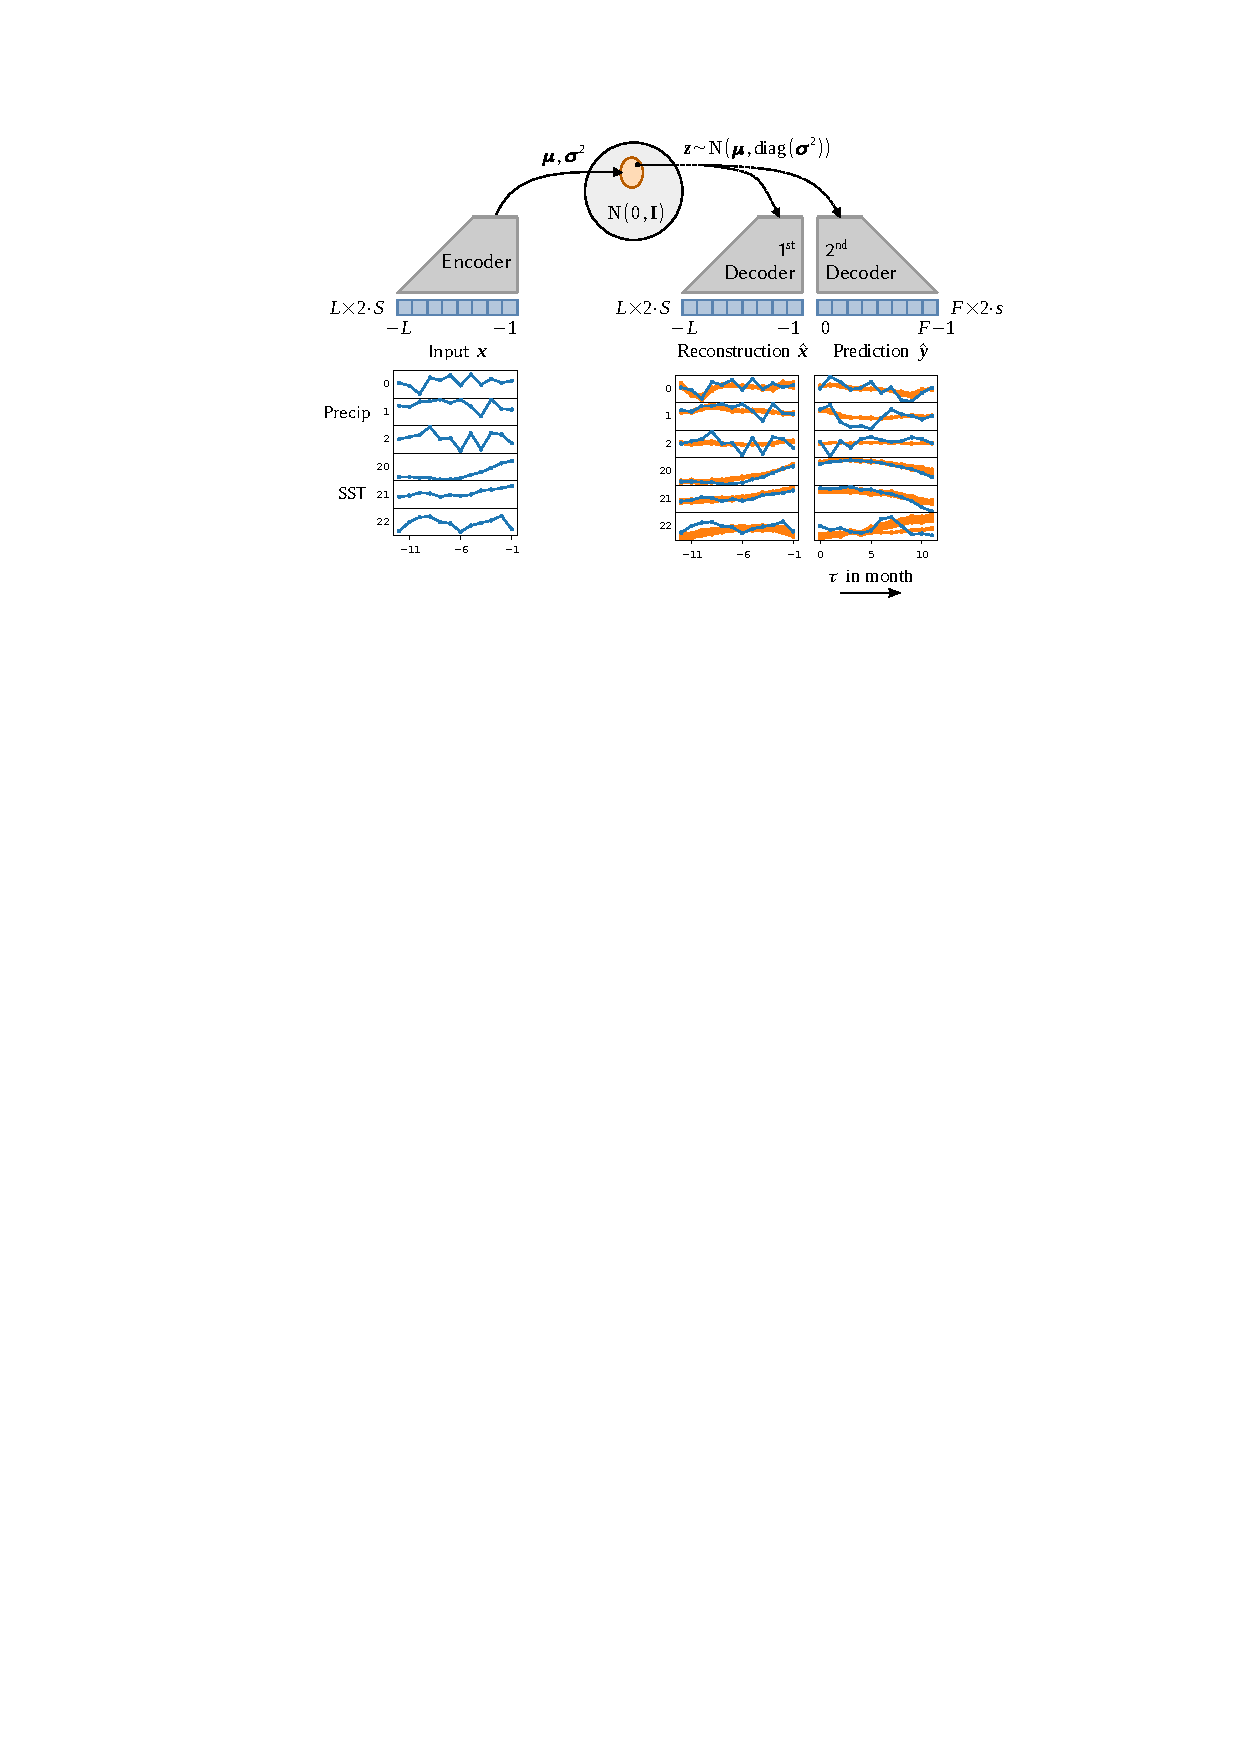
\includegraphics[width=0.8\linewidth]{Fig1_model_overview.pdf}
    \caption{\label{fig:model-overview}
        Overview of the model components. As in \cite{Groth.precip-predict.2023}, the model is a combination of a VAE, with its encoder (left) and decoder (middle), and a second decoder for prediction (right). An example of the input $\mathbf{x}$ to the encoder (blue) and the resulting stochastic reconstruction $\mathbf{\hat{x}}$ and prediction $\mathbf{\hat{y}}$ (orange) are shown below the corresponding model parts. With a prior $\mathcal{N}(0,\mathbf{I})$ over the latent space, the encoder approximates a posterior $\mathcal{N}(\boldsymbol{\mu},\mathrm{diag}(\boldsymbol{\sigma}^{2}))$, which is used by the two decoders to stochastically estimate the input $\mathbf{x}$ and prediction target $\mathbf{y}$ (blue).}
\end{figure}

The VAE combines variational inference with deep learning and provides a probabilistic approach to describe observations in the latent space \citep{Kingma.Welling.2014,Kingma.Welling.2019}. The VAE encoding and decoding methodology provides a computationally efficient way to a) infer information about latent variables from observations and b) to approximate the difficult-to-compute probability density functions (PDFs) that underlie the complex nonlinear dynamics in the multi-model CMIP ensemble.

To achieve this, the VAE is trained on samples from the multi-model dataset $\mathcal{D}=\{\mathcal{D}_{M}\}_{m=1}^{M}$ that combines the $M$ different SSP simulations, $\mathcal{D}_{m}=\{\mathbf{x}_{m}(n)\}_{n=1}^{N}$, each providing $N$ training samples (cf. Fig.~\ref{fig:model-overview}).

In contrast to \cite{Groth.precip-predict.2023}, here the VAE is trained on different SSP scenarios provided by the $M$ models. To incorporate the different SSP scenarios, we use the world CO$_2$ emissions of the different SSPs as auxiliary input to the VAE, which will be discussed in more detail in section~\ref{sec:model-architecture}.

The parameters of the VAE are likewise optimized by maximizing the \emph{evidence lower bound} (ELBO),
\begin{subequations}
    \begin{eqnarray}
        \mathcal{L}_{\mathrm{ELBO}}(\mathbf{x}) & = & \mathbb{E}_{q_{\phi}(\mathbf{z}|\mathbf{x})}\left[\log p_{\theta}(\mathbf{x}|\mathbf{z})\right] + \mathbb{E}_{q_{\phi}(\mathbf{z}|\mathbf{x})}\left[\log\left(\frac{p_{\theta}(\mathbf{z})}{q_{\phi}(\mathbf{z}|\mathbf{x})}\right)\right],\\
        & = & \mathbb{E}_{q_{\phi}(\mathbf{z}|\mathbf{x})}\left[\log p_{\theta}(\mathbf{x}|\mathbf{z})\right] - \mathrm{KL}\left(q_{\phi}(\mathbf{z}|\mathbf{x})\Vert p_{\theta}(\mathbf{z})\right),\label{eq:ELBO-components}
    \end{eqnarray}
\end{subequations}
i.e., the sum of a) the expected log-likelihood of the data $\mathbf{x}$, which is a measure of the reconstruction error of the decoder $p_\theta$, and b) the Kulback-Leibler (KL) divergence, which acts as a regularization term on the encoder $q_\phi$.

\subsection{Disentangled representations}

As in \cite{Groth.precip-predict.2023}, the ELBO objective is modified to improve the generalization capabilities of the VAE and to learn a more interpretable representation of the data. The modifications are identical to those in \cite{Groth.Chavez.2023} and reported in \cite{Groth.precip-predict.2023}. The modifications are the following:

\paragraph{$\beta$-VAE}
scales the KL term in Eq.~\eqref{eq:ELBO-components} and thus the regularization of the encoder \citep{Higgins.Matthey.ea.2017}.

\paragraph{Total correlation}
minimization encourages the encoder to learn more independent latent factors \citep{Chen.Li.ea.2018}.

\paragraph{Cross entropy}
minimization increases the diversity in the data generating process as well, i.e., to avoid overfitting the training data and to improve the generalization of the model \citep{Radford.Kim.ea.2021}.

\paragraph{Batch ensemble}
augmentation with different ensemble members is used to increase the chance of finding a disentangled representation, and to reduce the influence of randomness in the form of initial values of the model parameters and the training run \citep{Wen.Tran.ea.2020}.

In our experiments with the VAE, we found that the $\beta$-VAE and total correlation regularization terms are the most important ones to achieve a disentangled representation of the different SSP scenarios. The cross entropy and batch ensemble augmentation terms are less important, but still improve the generalization capabilities of the model. The hyperparameters of the VAE are described in more detail in section~\ref{sec:model-params-training}.

\subsection{VAE and forecasting}

As in \cite{Groth.precip-predict.2023}, the encoder and decoder are both implemented as feed-forward NNs and the approximate posterior is assumed to be a factorized Gaussian distribution. In addition to the auto-encoding task, a second decoder NN is trained on a prediction target. Similarly to the first decoder NN, the second decoder NN likewise samples from the approximate posterior. Their parameters $\theta$, $\phi$, and $\eta$ are optimized by minimizing the same loss function as in \cite{Groth.precip-predict.2023}:
\begin{multline}
    \mathcal{L}{}_{\theta,\phi,\eta}(\mathbf{x},\mathbf{y})=\mathbb{E}_{q_{\theta}(\mathbf{z}|\mathbf{x})}\left\Vert \mathbf{x}-\hat{\mathbf{x}}\right\Vert {}^{2}+\alpha\,\mathbb{E}_{q_{\theta}(\mathbf{z}|\mathbf{x})}\left\Vert \mathbf{y}-\hat{\mathbf{y}}\right\Vert {}^{2}\\
    +\beta\left[\mathrm{KL}\left(q_{\phi}(\mathbf{z}|\mathbf{x})\Vert p_{\theta}(\mathbf{z})\right)+\gamma\,\mathcal{L}_{\mathrm{TC}}(\mathbf{x})+\delta_{x}\mathcal{L}_{\mathrm{CE}}(\hat{\mathbf{x}})+\delta_{y}\,\mathcal{L}_{\mathrm{CE}}(\mathbf{\hat{y}})\right].\label{eq:total-loss}
\end{multline}
The first and second terms of Eq.~\eqref{eq:total-loss} represent the reconstruction and prediction error, respectively. The remaining term of Eq.~\eqref{eq:total-loss}, on the other hand, represent the various regularization penalties for the model; i.e. the Kulback-Leibler (KL) divergence between the approximate posterior and the prior, the total correlation (TC) term, and the two cross-entropy (CE) terms. A summary of their individual scaling parameters is provided in Section~\ref{sec:model-params-training}. To help the training, an annealing scheme is applied to the regularization strength in which the scale $\beta$ is gradually increased \citep{Bowman.Vilnis.ea.2015}.

The principles of the model design are the same as in \cite{Groth.precip-predict.2023} and only adapted to the new data. Figure~\ref{fig:model-overview} provides an overview of the different components of the model as well as of their interaction.  Below each of the parts, an example of the data is shown to illustrate the general flow of data within the model. The encoder receives as input a sample $\mathbf{x}\in\mathbb{R}^{L\times 2 \cdot S}$ from the CMIP data in section~\ref{sec:data}, combining values of the leading $S$ SST PCs with rainfall PCs in a sliding time window of length $L$. These are the observations of the last $L$ month before a given time $t$, which are used as input to the encoder NN to approximate the posterior $\mathcal{N}(\boldsymbol{\mu},\mathrm{diag}(\boldsymbol{\sigma}^{2}))$ at time $t$. The decoder NN samples from the posterior, $\mathbf{z}=\mathbf{z}(t)$, and provides stochastic reconstructions $\mathbf{\hat{x}}$ of past observations in the input $\mathbf{x}$, while the forecast NN provides stochastic predictions of the following $F$ months.

By jointly training the model in Fig.~\ref{fig:model-overview} on different SSP scenarios, the VAE learns a disentangled representation of the underlying temporal dynamics in the latent space that is invariant to the scenarios. To support the model in learning a latent represention that is invariant to the particular scenario, we provide auxiliary information about the forcing, cf. Section~\ref{sec:data}. This allows us sample from the posterior given the input data of any scenario and to decode it with the decoder NN into another scenario by manipulating the auxiliary input. Finally, this invariance allows us to make predictions about the data distribution underlying the newly synthesized scenarios. Given a sufficient number of widely varying scenarios, the model can learn to generalize to new scenarios within the boundaries of the training data.

\section{Model architecture of encoder and decoder NNs}\label{sec:model-architecture}

\begin{figure}
    \centering{}
    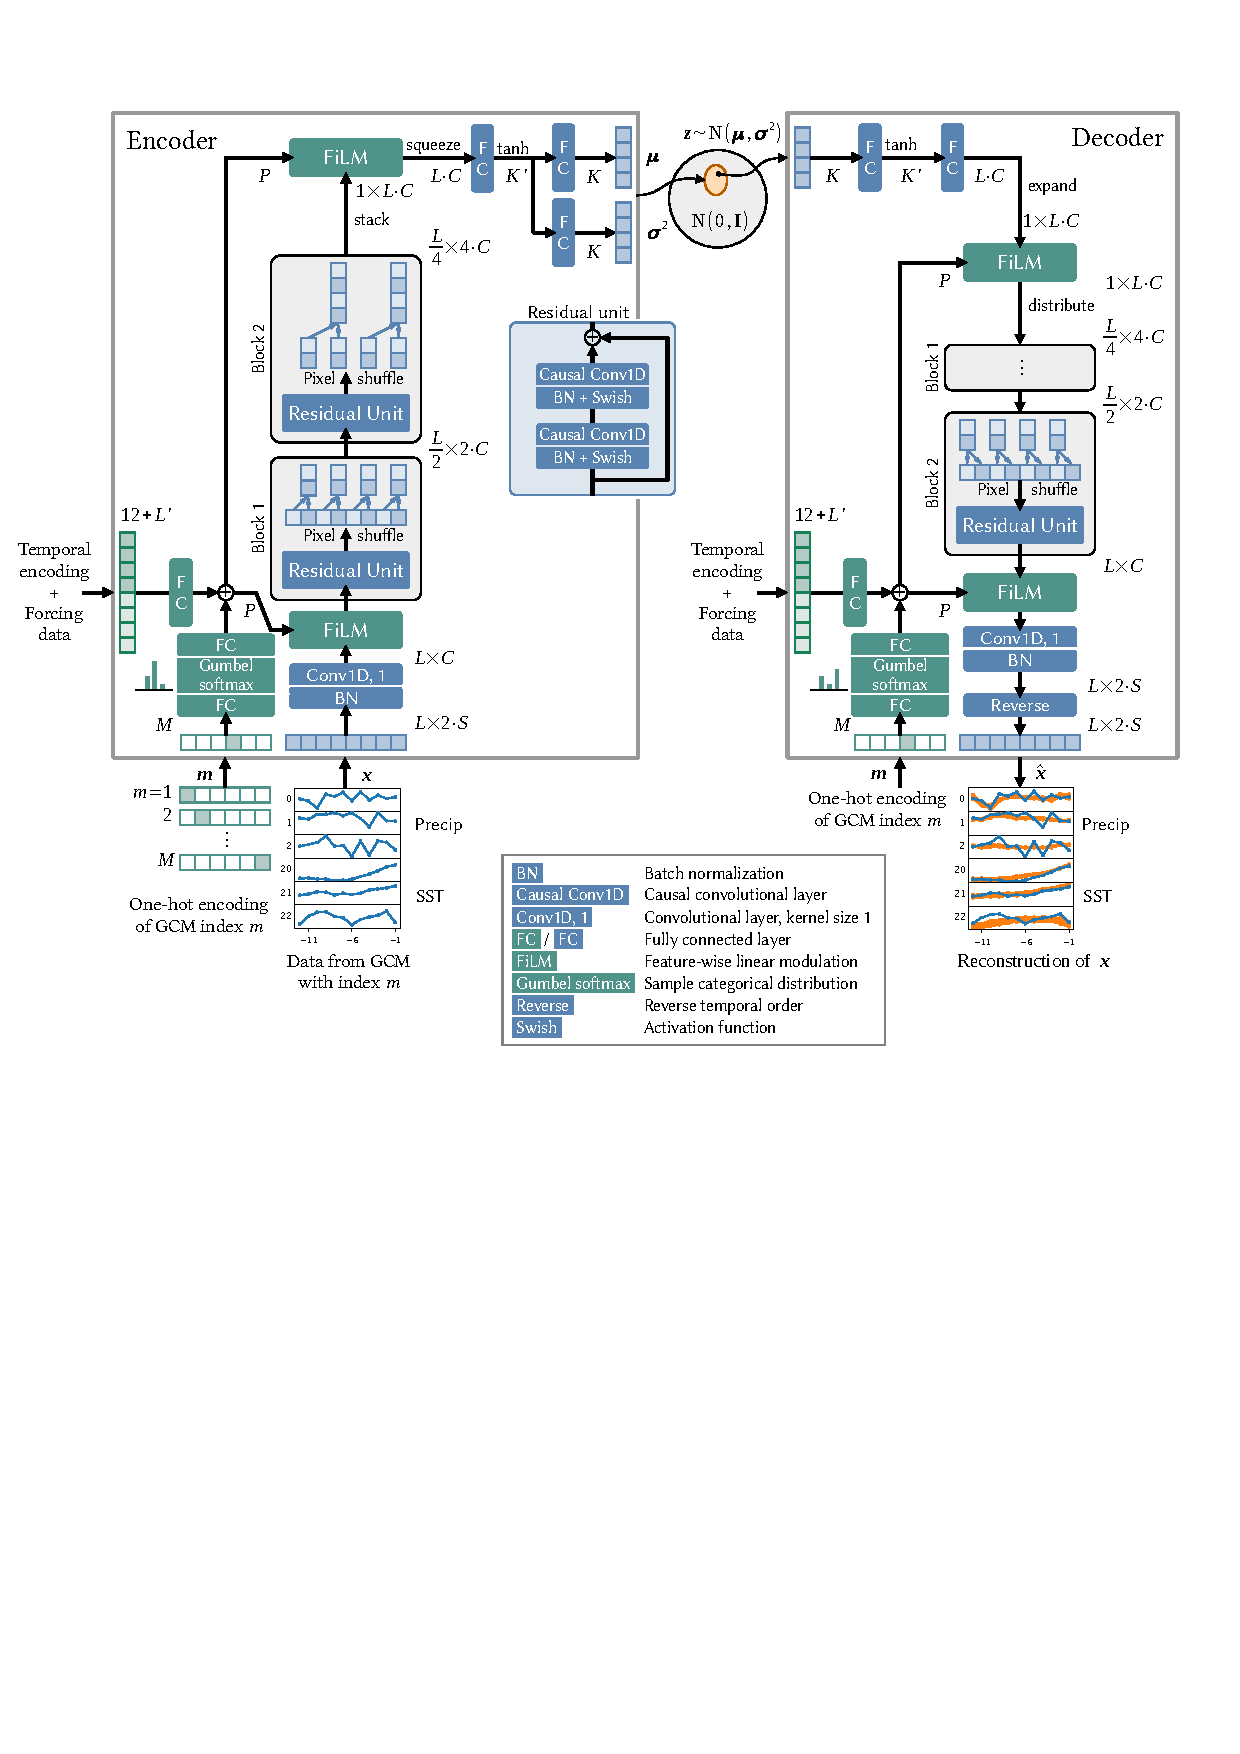
\includegraphics[width=\linewidth]{Fig2_model_details.pdf}
    \caption{\label{fig:model-details}Architecture of the encoder NN (left) and the decoder NN (right). The architure is identical to that of \cite{Groth.precip-predict.2023}. The figure shows the case of $B=2$ blocks. Examples of the input data $\mathbf{x}$ to the encoder and the decoder output $\mathbf{\hat{x}}$ are shown below the corresponding parts. The encoder and decoder consist of multiple blocks combining causal convolutional layers and resampling layers (blue boxes) to aggregate and distribute temporal information. The auxiliary input of the GCM index $m$ and the temporal information are used to modify intermediate features in the encoder and decoder NNs by FiLM layers (green boxes). Only the first decoder NN for reconstruction is shown, cf. Fig.~\ref{fig:model-overview}. The second decoder NN used for forecasting (not shown here) has the same structure and keeps the temporal order, i.e. has no reverse layer. Information on the world CO$_2$ concentration (forcing data) is provided together with temporal encoding as input to a FC layer, which is combined with the output of the Gumbel softmax sampling.}
\end{figure}

The following section provides a summary of the implementation details of the encoding and decoding NNs as introduced in \cite{Groth.Chavez.2023}; cf. also Fig.~\ref{fig:model-details}. The model design is identical to that in \cite{Groth.precip-predict.2023} and we refer to the latter for a more detailed description of the model architecture.

Similar to the model setup in \cite{Groth.precip-predict.2023}, the computation in the stack of residual blocks is influenced by so-called FiLM layers that modify the computation in the residual blocks based on auxiliary conditioning information via a simple, Feature-wise Linear Modulation \citep[FiLM,][]{Perez.Strub.ea.2018}.

In \cite{Groth.Chavez.2023} and also in \cite{Groth.precip-predict.2023}, the VAE is conditioned on two types of information: a) temporal information on the current month and b) ensemble information on the current ensemble member. In this report, we add a third type of conditioning information: c) information on the world CO$_2$ concentration.

To encode temporal information on the current month at time $t$, sine and cosine functions of different frequencies are combined,
\begin{equation}
    \mathbf{s}(t)=\left\{ \left(\sin(2\pi\frac{k}{12}t),\cos(2\pi\frac{k}{12}t)\right),\quad k=1,2,\dots,6\right\}.\label{eq:temporal-encoding}
\end{equation}
Provided as auxiliary input to the the VAE encoder and decoder, the temporal encoding allows them to seasonally adjust their computations.

To encode information about the current ensemble member, a random number from a categorical distribution is drawn, where the different categories represent different members of the batch ensemble. Conditioning on the ensemble member index $m$ allows the encoder and decoder to learn a distribution of the feature-wise scale and bias parameters in the FiLM layers that are specific to each of the $M$ CMIP models.

To encode information on the world CO$_2$ concentration, we provide the current and past values of the CO$_2$ concentration prior to time $t$. The CO$_2$ concentration data is provided on an annual time scale and we use the past $L'$ years of data as input to the VAE. During training, the same CO$_2$ concentration data is provided as auxiliary input to the encoder and decoder that corresponds to the input and target data. During inference, different values of CO$_2$ concentration data are provided as input to the decoder, which allows the VAE to generate forecasts for different CO$_2$ concentration scenarios while sampling from the latent space.

\section{Model configuration and training}\label{sec:model-params-training}

A summary of the exact values of the different model parameters of the VAE can be found in Table \ref{tab:model-params}. In total, the VAE has about 621\,k trainable parameters.
\begin{table}
    \caption{\label{tab:model-params}Summary of model configurations of encoder, decoder NNs as described in section~\ref{sec:model-architecture} and shown in Figs.~\ref{fig:model-overview} and \ref{fig:model-details}.}
    \centering{}
    \begin{tabular}{lcc}
        \toprule
        Parameter                    &             & Value        \\
        \midrule
        \# of input channels (PCs)   & $2 \cdot S$ & $2 \cdot 20$ \\
        Input length (month)         & $L$         & 12           \\
        Prediction length (month)    & $F$         & 12           \\
        Forcing input length (years) & $L'$        & 16           \\
        Embedding channels           & $C$         & 64           \\
        Residual blocks              & $B$         & 2            \\
        FC units                     & $K'$        & 96           \\
        Latent dimensions            & $K$         & 32           \\
        Size of batch ensemble       & $E$         & 6            \\
        Size of condition            & $P$         & 24           \\
        \midrule
        \# of model weights          &             & 621\,k       \\
        \bottomrule
    \end{tabular}
\end{table}

The training configuration is summarized in table \ref{tab:model-training}. The model weights are optimized using the Adam optimizer \citep{Kingma.Ba.2014} and a fixed learning rate $l_r$. They are optimized on the objective in Eq.~\eqref{eq:total-loss} with stochastic gradient descend on mini-batches of size $N_{\mathcal{M}}$. The mini-batches are augmented with $r$ different members sampled from the batch ensemble so that the different members are jointly optimized on the same data. The model is trained on the dataset of CMIP6 data for 25 epochs with a learning rate $l_r=1 \cdot 10^{-3}$.

\begin{table}
    \caption{\label{tab:model-training}Overview of the training configuration used in stochastic gradient descent and the corresponding scale parameters of the different loss terms in Eq.~\eqref{eq:total-loss}.}
    \centering{}
    \begin{tabular}{lccc}
        \toprule
        Parameter                    &                          & Value             \\
        \midrule
        \# training samples          &                          & 140\,k            \\
        \# of trained model weights  &                          & 621\,k            \\
        Batch size                   & $N_{\mathcal{M}}$        & 128               \\
        Ensemble members in batch    & $r$                      & 5                 \\
        Augmented batch size         & $r\cdot N_{\mathcal{M}}$ & 640               \\
        Learning rate                & $l_r$                    & $1 \cdot 10^{-3}$ \\
        Epochs                       &                          & 25                \\
        \midrule
        Scale of regularization      & $\beta$                  & $0\rightarrow50$  \\
        Scale of TC term             & $\gamma$                 & 5                 \\
        Scale of CE term in decoder  & $\delta_{x}$             & 1                 \\
        Scale of CE term in forecast & $\delta_{y}$             & 1                 \\
        Scale of prediction loss     & $\alpha$                 & 1                 \\
        \bottomrule
    \end{tabular}
\end{table}

We found that an increase in the regularization strength helps the VAE to improve the generalization of the latent space and to learn an disentangled representation that is invariant to the different scenarios. Therefore, we increase the regularization strength $\beta$ from 0 to 50 during training, which is an order of magnitude larger than the regularization strength used in \cite{Groth.precip-predict.2023}.


\section{Results}\label{sec:results}
This section presents first results of the VAE model and the future projection of precipitation for the crop seasons from 2014 to 2100.  We consider the crop season of soybean which is taken from the GGCMI crop calendar Phase 3 dataset \citep{Jaegermeyr.Mueller.ea.2021}.

\begin{figure}
    \centering
    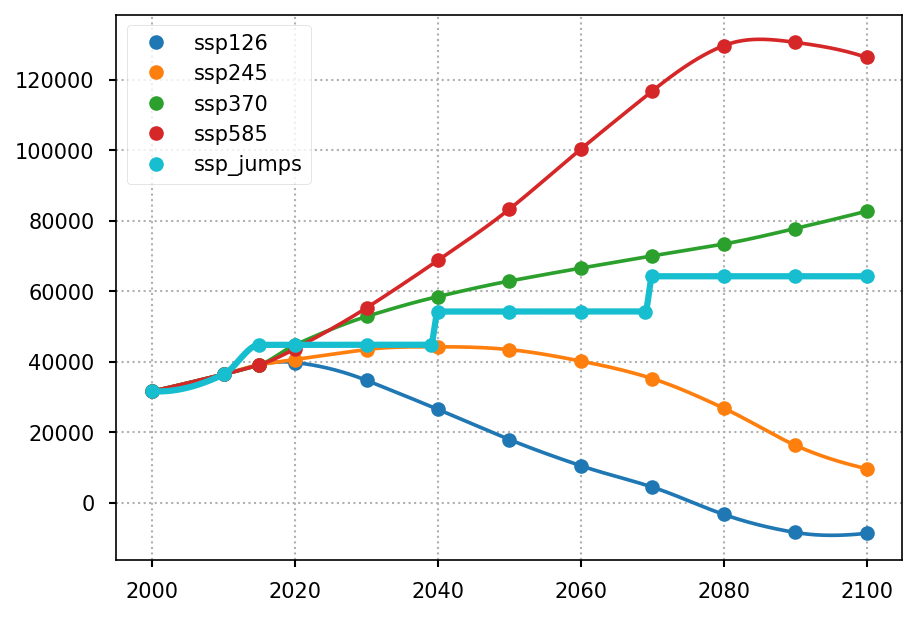
\includegraphics[width=0.45 \textwidth]{forcing}
    \caption{\label{fig:forcing}
        World CO$_2$ emission data (in Mt CO2/yr) used as input to the VAE. The figure compares the CO$_2$ concentration data from the different SSP scenarios (SSPs 126, 245, 370, 585) with the modified CO$_2$ concentration data (SSP jumps) used as input to the VAE.}
\end{figure}
In Fig.~\ref{fig:forcing}, we show the CO$_2$ concentration data used as input to the VAE. The figure compares the CO$_2$ concentration data from the different SSP scenarios with the modified CO$_2$ concentration data used as input to the VAE. This allows us to make future projections of precipitation for the crop seasons from 2014 to 2100 for a different CO$_2$ concentration scenario than originally used in the CMIP6 data. For demonstration purposes, we consider here a piecewise constant CO$_2$ concentration scenario, in which the CO$_2$ concentration is kept constant for 25 years and then stepwise increased by 10\,000 Mt/year.

\begin{figure}
    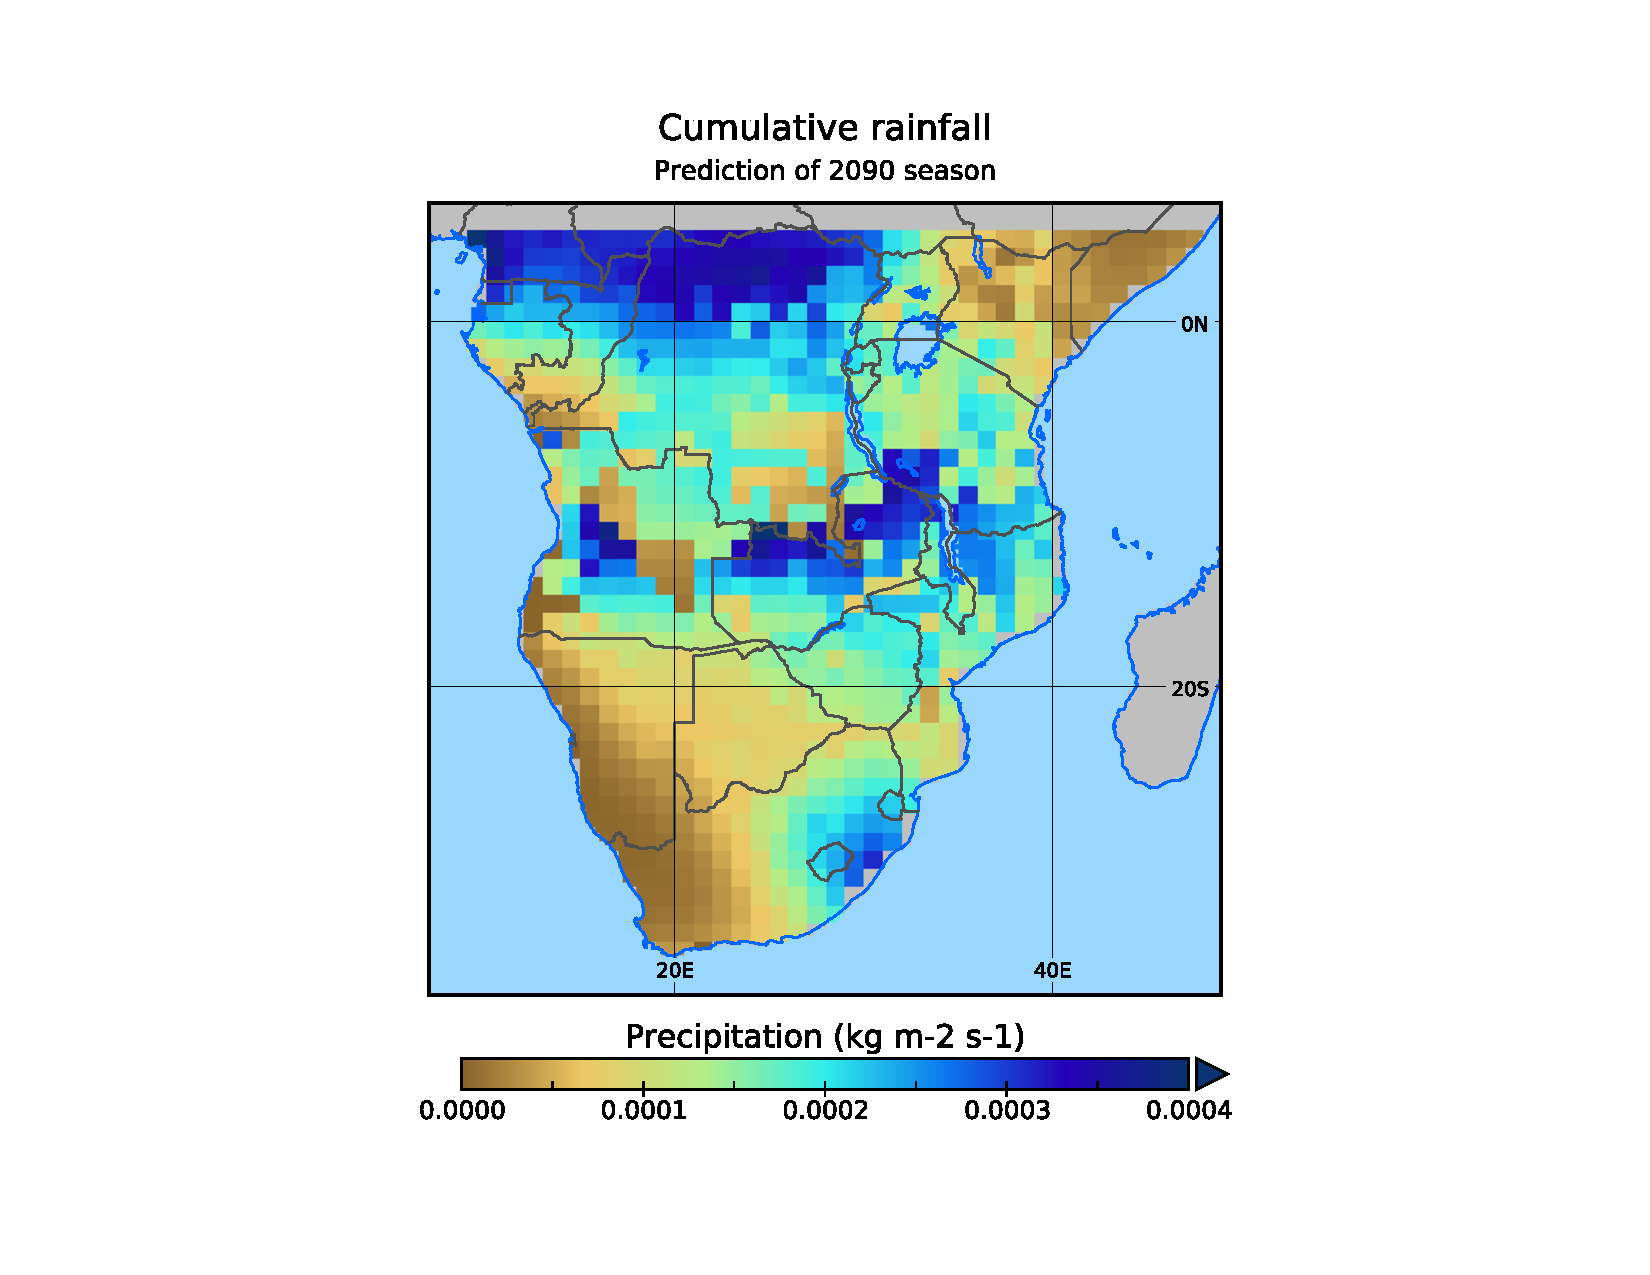
\includegraphics[width=0.49 \textwidth]{cum_pr.ensmedian.2090}
    \hfill
    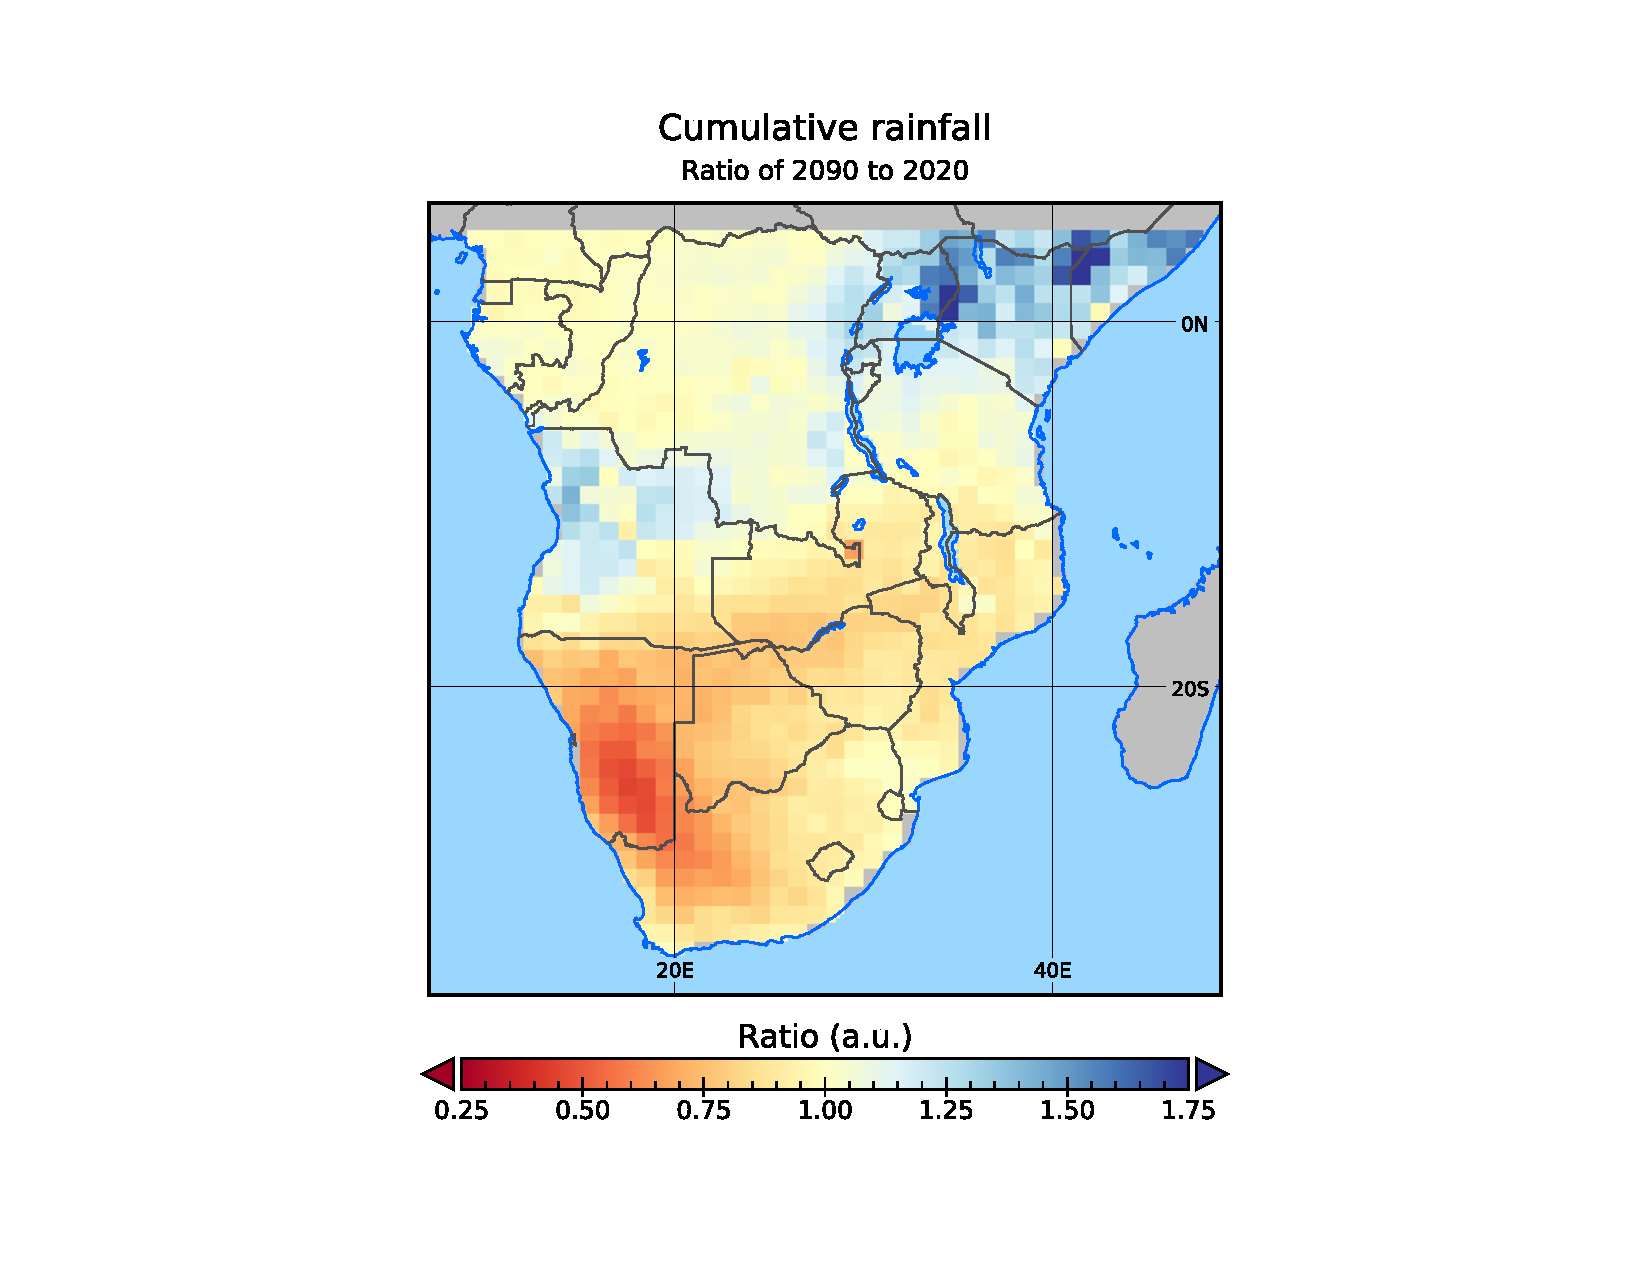
\includegraphics[width=0.49 \textwidth]{cum_pr.ensmedian.ratio}
    \caption{\label{fig:precip-prediction-map}
        Left: map of cumulative rainfall for the crop season of soybean in the year 2090. Right: ratio of crop seasons of soybean between the year 2090 and 2020 for the modified CO$_2$ concentration scenario (SSP jumps in Fig.~\ref{fig:forcing}). Dates for the crop season taken from the GGCMI crop calendar Phase 3 dataset \citep{Jaegermeyr.Mueller.ea.2021}.}
\end{figure}
In Fig.~\ref{fig:precip-prediction-map}, we show the predicted rainfall for the crop season in the year 2090 (left panel) and compare it with the crop season in 2020 (right panel). The overall picture is that the rainfall is predicted to decrease in most regions of Africa, while the decrease in rainfall in the southern part of Africa is particularly pronounced in the south-western part of Africa. On the other hand, it is interesting to note that we observe a few regions in the northern-eastern part of Africa where the rainfall is predicted to increase. However, these are regions where the rainfall is generally low (left panel).

\begin{figure}
    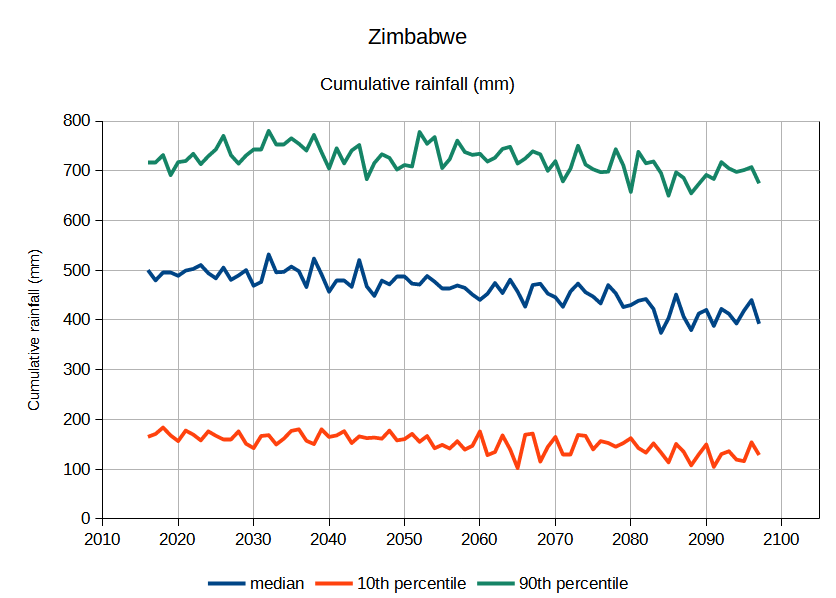
\includegraphics[width=0.49 \textwidth]{cum_precip.enspctl.ZW}
    \hfill
    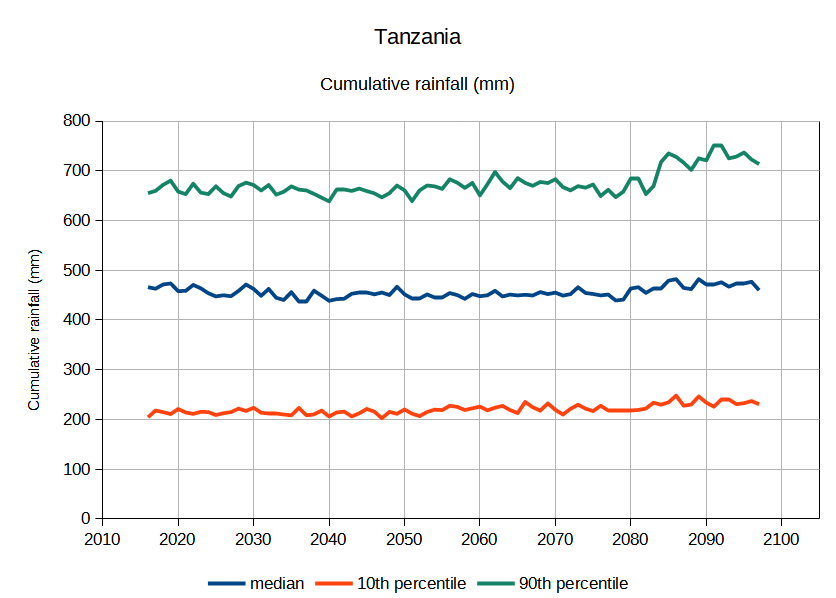
\includegraphics[width=0.49 \textwidth]{cum_precip.enspctl.TZ}
    \caption{\label{fig:precip-prediction-country}
        Country average of cumulative rainfall for the crop seasons of soybean from 2015 to 2100 for the modified CO$_2$ concentration scenario (SSP jumps in Fig.~\ref{fig:forcing}). Left: Zimbabwe. Right: Tanzania. The plot shows the median of the ensemble members and the 10\% and 90\% quantiles.}
\end{figure}
Next, we obtain the country averages of the predicted rainfall. The country averages obtained for Zimbabwe and Tanzania are shown in Fig.~\ref{fig:precip-prediction-country}. The plot shows the median and the 10\% and 90\% quantiles of the predicted distribution of rainfall while sampling from the posterior. The overall picture is that the rainfall is predicted to decrease in Zimbabwe, while the change in rainfall in Tanzania is less pronounced. In Zimbabwe, the decrease in rainfall is predicted to be more pronounced in the second half of the 21st century, such as we observe in many other regions of Africa, cf. again Fig.~\ref{fig:precip-prediction-map}. In Tanzania, the picture is more complex and is predicted to depend on the region. In the north-eastern part of Tanzania, the rainfall is predicted to increase, while in the south-western part of Tanzania, the rainfall is predicted to decrease. However, the change in rainfall is predicted to be less pronounced in Tanzania than in Zimbabwe.

\section*{Declarations}
\paragraph{Data and code availability}

The data and the Python scripts developed allowing to reproduce the experiments illustrated in this report are available at \url{https://github.com/andr-groth/VAE-SSP}.

\bibliographystyle{ametsoc2014}
\bibliography{VAE-SSP-biblio}


\end{document}
